% ============================================================
%   CHAPITRE : Variables aléatoires
%   Niveau   : Terminale S
%   Mazava Maths
% ============================================================
\chapter{Variables aléatoires}

\begin{objectifs}
	\begin{itemize}[label=\textbullet]
		\item Déterminer la loi de probabilité d'une variable aléatoire.
		\item Déterminer et représenter une fonction de répartition.
		\item Calculer et interpréter l'espérance, la variance et l'écart-type d'une variable aléatoire.
		\item Reconnaître une épreuve de Bernoulli et un schéma de Bernoulli.
	\end{itemize}
\end{objectifs}

On considère, tout au long de ce chapitre, l'exemple suivant : on lance deux pièces de monnaie équilibrées et on note $X$ le nombre de « Pile » obtenus.


% ============================================================
\section{Variable aléatoire et loi de probabilité}
% ============================================================

\begin{definition}[Variable aléatoire]
	Définir une \textbf{variable aléatoire} $X$ sur un univers $\Omega$, c'est associer un nombre réel à chaque issue de $\Omega$.

	L'ensemble des valeurs prises par $X$ est noté $X(\Omega)$.
\end{definition}

\begin{exemple}
	Pour le lancer des deux pièces, $\Omega = \{PP,\,PF,\,FP,\,FF\}$ et $X(\Omega) = \{0,1,2\}$ : $X=0$ si aucun Pile, $X=1$ si un seul Pile ($PF$ ou $FP$), $X=2$ si deux Piles.
\end{exemple}

\begin{definition}[Loi de probabilité]
	La \textbf{loi de probabilité} de $X$ associe à chaque valeur $x_i$ de $X(\Omega)$ la probabilité $p_i = \Prob(X=x_i)$. On la présente souvent sous forme d'un tableau, et on a toujours :
	\[
	\sum_i p_i = 1.
	\]
\end{definition}

\begin{exemple}
	Les quatre issues étant équiprobables :
	\begin{center}
		\begin{tabular}{|c|c|c|c|}
			\hline
			$x_i$ & $0$ & $1$ & $2$ \\
			\hline
			$\Prob(X=x_i)$ & $\dfrac14$ & $\dfrac12$ & $\dfrac14$ \\
			\hline
		\end{tabular}
	\end{center}
\end{exemple}

\begin{center}
	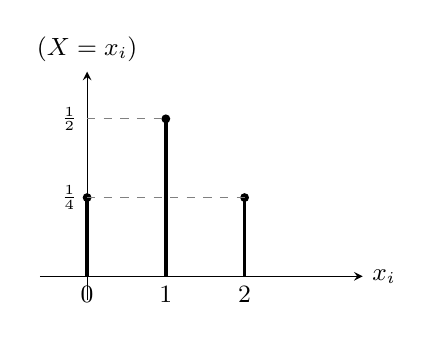
\begin{tikzpicture}[>=stealth, font=\small]
		\draw[->] (-0.6,0) -- (3.5,0) node[right] {$x_i$};
		\draw[->] (0,-0.3) -- (0,2.6) node[above] {$\Prob(X=x_i)$};
		\foreach \x/\h in {0/1, 1/2, 2/1}{
			\draw[very thick] (\x,0) -- (\x,\h);
			\fill (\x,\h) circle (1.6pt);
			\node[below] at (\x,0) {$\x$};
		}
		\draw[dashed, gray] (0,1) -- (2,1) (0,2) -- (1,2);
		\node[left] at (0,1) {\scriptsize $\frac14$};
		\node[left] at (0,2) {\scriptsize $\frac12$};
	\end{tikzpicture}
\end{center}


% ============================================================
\section{Fonction de répartition}
% ============================================================

\begin{definition}[Fonction de répartition]
	La \textbf{fonction de répartition} de $X$ est la fonction $F$ définie sur $\R$ par :
	\[
	F(x) = \Prob(X \leqslant x).
	\]
	C'est une fonction \textbf{croissante}, en escalier, qui vaut $0$ pour $x$ assez petit et $1$ pour $x$ assez grand.
\end{definition}

\begin{exemple}
	Pour l'exemple précédent : $F(x) = 0$ si $x<0$ ; $F(x) = \dfrac14$ si $0\leqslant x<1$ ; $F(x)=\dfrac34$ si $1\leqslant x<2$ ; $F(x)=1$ si $x\geqslant2$.
\end{exemple}

\begin{center}
	\begin{tikzpicture}[>=stealth, font=\small]
		\draw[->] (-1,0) -- (4,0) node[right] {$x$};
		\draw[->] (0,-0.3) -- (0,3.4) node[above] {$F(x)$};
		\draw[thick] (-1,0) -- (0,0);
		\draw[thick] (0,0.75) -- (1,0.75);
		\draw[thick] (1,2.25) -- (2,2.25);
		\draw[thick] (2,3) -- (3.5,3);
		\draw[dashed, gray] (0,0.75) -- (1,0.75) (0,2.25) -- (1,2.25) (0,3) -- (2,3);
		\draw[fill=black] (0,0.75) circle (1.6pt);
		\draw[fill=white] (1,0.75) circle (1.6pt);
		\draw[fill=black] (1,2.25) circle (1.6pt);
		\draw[fill=white] (2,2.25) circle (1.6pt);
		\draw[fill=black] (2,3) circle (1.6pt);
		\node[below] at (0,0) {$0$};
		\node[below] at (1,0) {$1$};
		\node[below] at (2,0) {$2$};
		\node[left] at (0,0.75) {\scriptsize $\frac14$};
		\node[left] at (0,2.25) {\scriptsize $\frac34$};
		\node[left] at (0,3) {\scriptsize $1$};
	\end{tikzpicture}
\end{center}

\begin{astucebac}
	Sur chaque intervalle, $F$ est constante et égale à la somme des probabilités déjà « rencontrées » ; elle « saute » de $p_i$ exactement en $x=x_i$, et le point plein (inclus) est toujours à droite du saut.
\end{astucebac}


% ============================================================
\section{Espérance, variance, écart-type}
% ============================================================

\begin{definition}[Espérance mathématique]
	L'\textbf{espérance mathématique} de $X$ est le nombre :
	\[
	\Esp(X) = \sum_i p_i\,x_i.
	\]
	Elle représente la valeur moyenne de $X$ que l'on peut espérer obtenir en répétant un grand nombre de fois l'expérience.
\end{definition}

\begin{definition}[Variance et écart-type]
	La \textbf{variance} de $X$ est le nombre :
	\[
	\Var(X) = \sum_i p_i\bigl(x_i-\Esp(X)\bigr)^2 = \left(\sum_i p_i x_i^2\right) - \bigl[\Esp(X)\bigr]^2.
	\]
	L'\textbf{écart-type} de $X$ est $\sigma(X) = \sqrt{\Var(X)}$. Ce sont des indicateurs de la \textbf{dispersion} de $X$ autour de son espérance.
\end{definition}

\begin{methode}
	\textbf{Calculer $\Esp(X)$, $\Var(X)$ et $\sigma(X)$ :}
	\begin{enumerate}
		\item Dresser le tableau de la loi de probabilité de $X$.
		\item Calculer $\Esp(X) = \sum p_i x_i$.
		\item Calculer $\sum p_i x_i^2$, puis $\Var(X) = \sum p_i x_i^2 - [\Esp(X)]^2$ (formule de König-Huygens).
		\item Calculer $\sigma(X) = \sqrt{\Var(X)}$.
	\end{enumerate}
\end{methode}

\begin{exemple}
	Pour l'exemple précédent :
	\[
	\Esp(X) = \frac14\times0 + \frac12\times1 + \frac14\times2 = 1.
	\]
	\[
	\sum p_i x_i^2 = \frac14\times0 + \frac12\times1 + \frac14\times4 = \frac32,
	\qquad
	\Var(X) = \frac32 - 1^2 = \frac12,
	\]
	\[
	\sigma(X) = \sqrt{\frac12} = \frac{\sqrt2}{2}.
	\]
\end{exemple}

\begin{propriete}{Linéarité de l'espérance}{}
	Pour tous réels $a$ et $b$ :
	\[
	\Esp(aX+b) = a\,\Esp(X)+b, \qquad \Var(aX+b) = a^2\,\Var(X).
	\]
\end{propriete}


% ============================================================
\section{Épreuve et schéma de Bernoulli}
% ============================================================

\begin{definition}[Épreuve de Bernoulli]
	Une \textbf{épreuve de Bernoulli} est une expérience aléatoire n'ayant que deux issues : un \textbf{succès} (de probabilité $p$) et un \textbf{échec} (de probabilité $1-p$).

	La variable aléatoire $X$ qui vaut $1$ en cas de succès et $0$ en cas d'échec suit la \textbf{loi de Bernoulli} de paramètre $p$, notée $\mathscr{B}(p)$.
\end{definition}

\begin{center}
	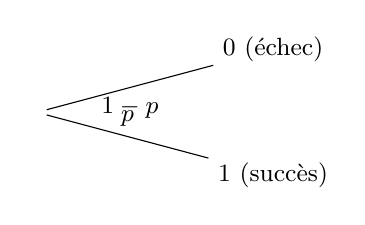
\begin{tikzpicture}[>=stealth, grow=right, level distance=3cm, sibling distance=1.6cm, font=\small]
		\node {}
		child { node {$1$ (succès)} edge from parent node[above] {$p$} }
		child { node {$0$ (échec)} edge from parent node[below] {$1-p$} };
	\end{tikzpicture}
\end{center}

\begin{propriete}{Espérance et variance d'une loi de Bernoulli}{}
	Si $X$ suit la loi $\mathscr{B}(p)$, alors :
	\[
	\Esp(X) = p \qquad \text{et} \qquad \Var(X) = p(1-p).
	\]
\end{propriete}

\begin{definition}[Schéma de Bernoulli]
	Un \textbf{schéma de Bernoulli} consiste à répéter $n$ fois, de façon \textbf{identique et indépendante}, la même épreuve de Bernoulli de paramètre $p$.
\end{definition}

\begin{exemple}
	On lance $n$ fois un dé équilibré et on considère comme succès l'événement « obtenir un $6$ » ($p=\frac16$). Répéter ce lancer $n$ fois de façon indépendante constitue un schéma de Bernoulli de paramètres $n$ et $\frac16$. Le nombre de succès obtenus sur les $n$ répétitions suivra une \textbf{loi binomiale} (chapitre suivant).
\end{exemple}


% ============================================================
\section{Exercices résolus}
% ============================================================

\exerciceresolu
\textbf{Déterminer une loi de probabilité et calculer $\Esp$, $\Var$, $\sigma$}

Un jeu consiste à lancer un dé équilibré à six faces. Si le joueur obtient $6$, il gagne $10$ points ; s'il obtient un multiple de $3$ autre que $6$ (c'est-à-dire $3$), il gagne $2$ points ; sinon il perd $1$ point. On note $X$ le gain algébrique du joueur.
\begin{enumerate}
	\item Déterminer la loi de probabilité de $X$.
	\item Calculer $\Esp(X)$. Le jeu est-il favorable au joueur ?
	\item Calculer $\Var(X)$ et $\sigma(X)$.
\end{enumerate}

\solution

\textbf{1.} $X(\Omega) = \{-1,2,10\}$ avec $\Prob(X=10)=\dfrac16$, $\Prob(X=2)=\dfrac16$ et $\Prob(X=-1)=\dfrac46=\dfrac23$ (les résultats $1,2,4,5$).

\begin{center}
	\begin{tabular}{|c|c|c|c|}
		\hline
		$x_i$ & $-1$ & $2$ & $10$ \\
		\hline
		$\Prob(X=x_i)$ & $\dfrac23$ & $\dfrac16$ & $\dfrac16$ \\
		\hline
	\end{tabular}
\end{center}

\textbf{2.} $\Esp(X) = \dfrac23\times(-1) + \dfrac16\times2 + \dfrac16\times10 = -\dfrac23+\dfrac13+\dfrac53 = \dfrac43$.

Comme $\Esp(X) > 0$, le jeu est en moyenne favorable au joueur.

\textbf{3.} $\displaystyle\sum p_i x_i^2 = \frac23\times1 + \frac16\times4 + \frac16\times100 = \frac23+\frac23+\frac{100}{6} = \frac{4+4+100}{6} = 18$.

\[
\Var(X) = 18 - \left(\frac43\right)^2 = 18-\frac{16}{9} = \frac{162-16}{9} = \frac{146}{9}, \qquad
\sigma(X) = \sqrt{\frac{146}{9}} = \frac{\sqrt{146}}{3}.
\]


% ============================================================
\section{Exercices}
% ============================================================

\exercice{Loi de probabilité simple \hfill \facile}

On lance un dé équilibré et on note $X$ le nombre obtenu si celui-ci est pair, et $0$ sinon.
\begin{enumerate}
	\item Déterminer $X(\Omega)$ et la loi de probabilité de $X$.
	\item Représenter cette loi par un diagramme en bâtons.
	\item Calculer $\Esp(X)$.
\end{enumerate}

\exercice{Fonction de répartition \hfill \moyen}

Une variable aléatoire $X$ prend les valeurs $-2$, $0$ et $3$ avec les probabilités respectives $0,2$ ; $0,5$ et $0,3$.
\begin{enumerate}
	\item Vérifier que ces données définissent bien une loi de probabilité.
	\item Déterminer et représenter la fonction de répartition $F$ de $X$.
	\item Calculer $\Esp(X)$, $\Var(X)$ et $\sigma(X)$.
\end{enumerate}

\exercice{Jeu de hasard \hfill \moyen}

On tire une boule dans une urne contenant $2$ boules rouges, $3$ boules vertes et $5$ boules jaunes. Une boule rouge fait gagner $5$ points, une boule verte fait gagner $1$ point, une boule jaune fait perdre $2$ points. Soit $X$ le gain obtenu.
\begin{enumerate}
	\item Déterminer la loi de probabilité de $X$.
	\item Calculer l'espérance de gain. Le jeu est-il équitable ?
\end{enumerate}

\exercice{Épreuve de Bernoulli \hfill \difficile}

Une urne contient $8$ boules indiscernables au toucher : $5$ blanches et $3$ noires. On tire une boule et on considère un succès si elle est blanche.
\begin{enumerate}
	\item Justifier qu'il s'agit d'une épreuve de Bernoulli et donner son paramètre $p$.
	\item Soit $X$ la variable de Bernoulli associée. Donner $\Esp(X)$ et $\Var(X)$.
	\item On répète cette épreuve $5$ fois, en remettant la boule tirée à chaque fois. S'agit-il d'un schéma de Bernoulli ? Justifier et préciser ses paramètres.
\end{enumerate}
